In terms of NUTS II regions, Portugal is divided in seven groups.
The structuring of the Portuguese territory according to the New Territorial Units for Statistical Purposes, NUTS 2013,  in application in the National Statistical System since 1 January 2015 is composed of seven NUTS II: North, Centre, Lisbon Metropolitan Area (AML), Alentejo and Algarve regions, on the mainland, and the two autonomous regions. \cite{INEE}
\begin{figure}[h]
\centering % para centralizarmos a figura
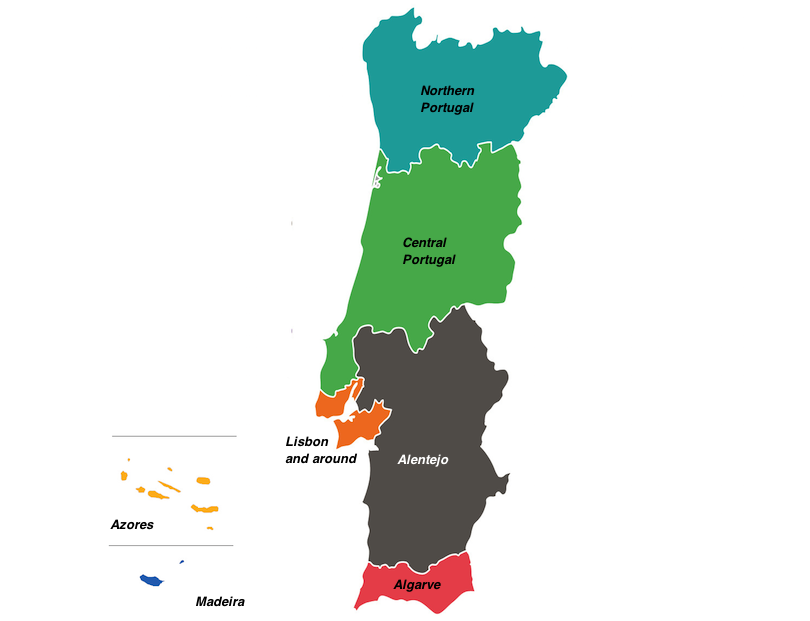
\includegraphics[width=10cm]{images/portugal.png} 

\caption{Portugal's Regions}
\label{figura:qualquernome}
\end{figure}

We'll describing them below, also mentioning some statistical data that may be interesting. \\
All information related to the labor market in the regions was obtained by consulting the  website of the European Commission \cite{trab}. The demographic percentages presented are based on data from  National Institute of Statistics of Portugal, INE. 

\subsubsection{North}
The employment structure in the North region presents 3 sub-regions with specific characteristics: 
The Porto Metropolitan Area, with a strong incidence of services (mainly trade) with greater technological and knowledge intensity. A surrounding shore, where industrial employment is  higher than the national average and rural areas, where nearly half of employment is concentrated in agriculture or non-commercial services.

In terms of {\textbf{demographics}}:
    \begin{itemize}
        \item Population density: {34,73\textdiscount} . 
        \item Gender: {47,2\textdiscount} male and {52,8\textdiscount} female.
        \item Age: 
        \begin{itemize}
        \item {12,63 \textdiscount} aged 14 and younger;
        \item {66,43\textdiscount} aged 15 to 64;
        \item {20,94\textdiscount} aged 65 and older.
        \end{itemize}
    \end{itemize}

\subsubsection{Center}
In this region, the Services sector is the most relevant in terms of employment - with emphasis on Trade and Vehicle Repair, Health and Social Support Services and the Education. \\
In terms of {\textbf{demographics}}:
    \begin{itemize}
        \item Population density: {21,54\textdiscount} . 
        \item Gender: {47,42\textdiscount} male and {52,58\textdiscount} female.
        \item Age: 
        \begin{itemize}
        \item {12,05 \textdiscount} aged 14 and younger;
        \item {63,42\textdiscount} aged 15 to 64;
        \item {24,53\textdiscount} aged 65 and older.
        \end{itemize}
    \end{itemize}
    
\subsubsection{Metropolitan area of Lisbon }
This is the region with the highest population density in the country. It's the region with the highest concentration of services, with emphasis on services provided mostly by the Public Sector; Education; Health and social support services.\\
In terms of {\textbf{demographics}}:
    \begin{itemize}
        \item Population density: {27,81\textdiscount} . 
        \item Gender: {46,71\textdiscount} male and {53,29\textdiscount} female.
        \item Age: 
        \begin{itemize}
        \item {15,88\textdiscount} aged 14 and younger;
        \item {62,04\textdiscount} aged 15 to 64;
        \item {22,08\textdiscount} aged 65 and older.
        \end{itemize}
    \end{itemize}
    
\subsubsection{Alentejo}
This is the region with the lowest population density in the country. Most of the region's territory is dedicated to Agriculture, allied to cattle breeding and also forestry.\\
In terms of {\textbf{demographics}}:

    \begin{itemize}
        \item Population density: {6,84\textdiscount} . 
        \item Gender: {47,97\textdiscount} male and {52,03\textdiscount} female.
        \item Age: 
        \begin{itemize}
        \item {12,4\textdiscount} aged 14 and younger;
        \item {62,05\textdiscount} aged 15 to 64;
        \item {25,55\textdiscount} aged 65 and older.
        \end{itemize}
    \end{itemize}
    
\subsubsection{Algarve}
The economic structure of this region is based on 5 strategic sectors associated with the region's natural resources: hospitality, catering and tourism, health, creative activities, agri-food and maritime activities. 
In terms of {\textbf{demographics}}:
    \begin{itemize}
        \item Population density: {34,73\textdiscount} . 
        \item Gender: {47,2\textdiscount} male and {52,8\textdiscount} female.
        \item Age: 
        \begin{itemize}
        \item {12,63\textdiscount} aged 14 and younger;
        \item {66,43\textdiscount} aged 15 to 64;
        \item {20,94\textdiscount} aged 65 and older.
        \end{itemize}
    \end{itemize}
    
\subsubsection{Azores autonomous region}
The region's economy is fundamentally based on activities mainly from the Public Sector (Public Administration, Social Security, Education, Health and Social Support activities). The activities of Trade and Repair of Vehicles and Accommodation and Restoration are equally important in employment in the region. \\
In terms of {\textbf{demographics}}:
    \begin{itemize}
        \item Population density: {2,36\textdiscount} . 
        \item Gender: {48,55\textdiscount} male and {51,45\textdiscount} female.
        \item Age: 
        \begin{itemize}
        \item {15,37\textdiscount} aged 14 and younger;
        \item {69,69\textdiscount} aged 15 to 64;
        \item {14,99\textdiscount} aged 65 and older.
        \end{itemize}
    \end{itemize}
    
\subsubsection{Madeira autonomous region }
In terms of more established work areas, this region is very similar to the Azores region. Tourism has an important role for both regions.\\
In terms of {\textbf{demographics}}:
    \begin{itemize}
        \item Population density: {2,47\textdiscount} . 
        \item Gender: {46,67\textdiscount} male and {53,33\textdiscount} female.
        \item Age: 
        \begin{itemize}
        \item {13,11\textdiscount} aged 14 and younger;
        \item {69,91\textdiscount} aged 15 to 64;
        \item {16,98\textdiscount} aged 65 and older.
        \end{itemize}
    \end{itemize}



